\section{Energetyka Jądrowa}

\begin{columnframe}{Dlaczego energetyka jądrowa może być rozwiązaniem?}
    \begin{column}{0.5\textwidth}
        \begin{figure}
            \centering
            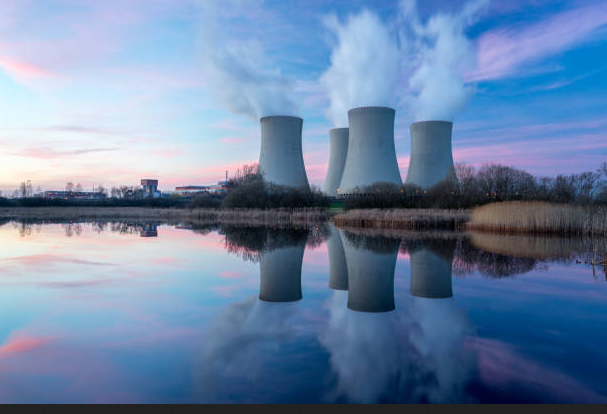
\includegraphics[width=0.6\textwidth, frame]{images/nuclear_powerplant_shutterstock.png}
        \end{figure}
    \end{column}
    \begin{column}{0.5\textwidth}
        \begin{itemize}
            \item Magazynowanie CO2 wymaga dużo energii oraz ciepła
            \item Temperatura osiągalna w reaktorach jądrowych pozwala na rozszczepienie wody (o czym więcej za chwilę)
        \end{itemize}
    \end{column}
\end{columnframe}


\begin{columnframe}{Reaktory HTR (High Temperature Reactor)}
    \begin{column}{0.5\textwidth}
        \begin{figure}
            \centering
            
\includegraphics[width=0.6\textwidth, frame]{images/pusheen.png}
        \end{figure}
    \end{column}
    \begin{column}{0.5\textwidth}
        \begin{itemize}
            \item one \keV
            \item two \MeV
            \item three \GeV
            \item \aegis
        \end{itemize}
    \end{column}
\end{columnframe}

\begin{columnframe}{Koszty produkcji energii jądrowej na tle innych źródeł}
    \begin{column}{0.5\textwidth}
        \begin{figure}
            \centering
            
\includegraphics[width=0.6\textwidth, frame]{images/pusheen.png}
        \end{figure}
    \end{column}
    \begin{column}{0.5\textwidth}
        \begin{itemize}
            \item one \keV
            \item two \MeV
            \item three \GeV
            \item \aegis
        \end{itemize}
    \end{column}
\end{columnframe}


\begin{columnframe}{Energetyka jądrowa w kontekście SJW}
    \begin{column}{0.5\textwidth}
        \begin{figure}
            \centering
            
\includegraphics[width=0.6\textwidth, frame]{images/pusheen.png}
        \end{figure}
    \end{column}
    \begin{column}{0.5\textwidth}
        \begin{itemize}
            \item one \keV
            \item two \MeV
            \item three \GeV
            \item \aegis
        \end{itemize}
    \end{column}
\end{columnframe}

\begin{columnframe}{Obecne źródła energii i ich emisyjność}
    \begin{column}{0.5\textwidth}
        \begin{figure}
            \centering
            
\includegraphics[width=0.6\textwidth, frame]{images/pusheen.png}
        \end{figure}
    \end{column}
    \begin{column}{0.5\textwidth}
        \begin{itemize}
            \item one \keV
            \item two \MeV
            \item three \GeV
            \item \aegis
        \end{itemize}
    \end{column}
\end{columnframe}

\begin{columnframe}{Role energetyki jądrowej w miksie energetycznym}
    \begin{column}{0.5\textwidth}
        \begin{figure}
            \centering
            
\includegraphics[width=0.6\textwidth, frame]{images/pusheen.png}
        \end{figure}
    \end{column}
    \begin{column}{0.5\textwidth}
        \begin{itemize}
            \item one \keV
            \item two \MeV
            \item three \GeV
            \item \aegis
        \end{itemize}
    \end{column}
\end{columnframe}
